\documentclass[10pt,twocolumn,letterpaper]{article}
\usepackage{cvpr}
\usepackage{times}
\usepackage{graphicx}
\usepackage{amsmath}
\usepackage{amssymb}
\usepackage[pagebackref=true,breaklinks=true,colorlinks,bookmarks=false]{hyperref}
\begin{document}
\title{311-Service-Request Data Analysis using Apache Spark - SOEN 691 Project}
\author{Apoorv Semwal \and Hareesh Kavumkulath \and Loveshant Grewal}
\maketitle

\begin{abstract}
Recent advances in the field of Big Data Analytics and Machine Learning have introduced a plethora of open-source tools and technologies for both, 
academia and the growing data analyst community. In this project we try leveraging one such popular distributed data processing framework Apache Spark
to analyse 311 - Service Request Data for the city of New-York. Being updated almost on a daily basis for the last 10 years, massive size of this dataset makes it a suitable candidate for analysis using a distributed data processing framework like Spark. Making use of Spark Ecosystem libraries like Spark SQL and Spark ML, on this dataset, enables us to derive some interesting insights, which might drive better resource planning within the city. Identifying the 3 primary goals for this project we first try answering a few statistical questions like “most frequent complaints reported(across entire city/borough wise)”, “Average time to resolve the request (category/department wise)”, “mostly used source for making request(borough wise)” and “most busy days/months in terms of request volumes”.
Arriving at these statistical figures involve making extensive use of Spark SQLs Dataframe API. Secondly we generate a model for predicting the closure time for any new incoming service request, after comparing performance of a set of selected supervised learning algorithms available in Spark ML. As part of our last goal we would be applying K-Means clustering over a selected set of features dividing the dataset into clusters to further analyse them for identifying any underlying service request patterns.
\end{abstract}

\section{Introduction}

\section{Section 2}

\textbf{1. Sample 1:} Its some random text:
\begin{itemize}
  \item Sample Item 1 \textbf{{\em Sample Italics}} in the dataset.
  \item Sample Item 1 \textbf{{\em Italics}}, 
\end{itemize}

\textbf{2. Sample 2:}\\
\begin{tabular}{ |p{3cm}|p{5cm}|  }
 \hline
 \multicolumn{2}{|c|}{Sample Table} \\
 \hline
 Sample1 &Sample\_1, Sample\_2, Sample\_3\_1\\
 \hline
 Sample1 &Sample\_1, Sample\_2, Sample\_3\_1\\
 \hline
 Sample1 &Sample\_1, Sample\_2, Sample\_3\_1\\
 \hline
\end{tabular}\\

\begin{figure}
   \begin{center}
  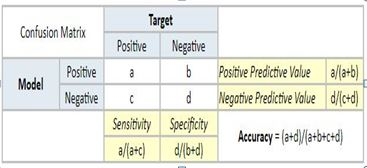
\includegraphics[width=\linewidth]{ConfusionMatrix.JPG}
   \end{center}
   \caption{Sample Confusion Matrix.\cite{W1}
   \label{Img1}}
\end{figure} 
Sample Reference of a figure in text. Figure~\ref{Img1}.\\

\begin{tabular}{ |p{0.5cm}||p{1.4cm}|p{1.4cm}|p{1.4cm}|p{1.4cm}|  }
 \hline
 \multicolumn{5}{|c|}{Multicol Table} \\
 \hline
 ID & Sample2 & Sample3 & Sample4 & Sample5\\
 \hline
 1 & 74.5 & 64.5 & 63.5 & 66.0\\
 \hline
 2 & 78.41 & 81.61 & 81.81 & 82.95\\
 \hline
\end{tabular}\\

\begin{equation}
\frac{\partial Sample Equation_{y_i}}{\partial X}
\end{equation}

\section{Conclusions}
\appendix
{\small
\bibliographystyle{cvpr_bibstyle}
\bibliography{bibliography}
}
\end{document}